 \documentclass[12pt,a4paper]{article}
\usepackage[utf8]{inputenc}
\usepackage{geometry}
\geometry{left=25mm,right=25mm,top=25mm,bottom=25mm}
\usepackage{times}
\usepackage{amsmath,amssymb}
\usepackage{graphicx}
\usepackage{caption}
\usepackage{subcaption}
\usepackage{booktabs}
\usepackage{multicol}
\usepackage{float}
\usepackage{hyperref}
\usepackage{tikz}
\usetikzlibrary{shapes.geometric, arrows.meta, positioning}
\usepackage{pgfplots}
\pgfplotsset{compat=1.17}
\usepackage{algorithmic}
\usepackage[ruled,vlined]{algorithm2e}

\title{Intelligent Condition Based Monitoring Using
Acoustic Signals for Air Compressors\\
\vspace{6pt}
\large A concise report based on Verma \textit{et al.}, IEEE Trans. on Reliability (2016)}
\author{Srinjoy Chakraborty}
\date{\today}
\begin{document} % <-- must come first
\maketitle % generates the title
\newpage
\tableofcontents % table of contents
\listoffigures % table of figures
\newpage
\begin{multicols}{2}
\section{Abstract}
Early detection of machine faults is vital to prevent costly downtime and ensure workplace safety, as the source is \cite{Verma2016}. This paper presents a practical, data-driven process for building acoustic-based fault-diagnosis systems for reciprocating air compressors. The proposed pipeline is deliberately end-to-end: it covers how to collect acoustic data, how to choose the best microphone location, how to clean and normalize the recordings, which time/frequency/time–frequency features to extract, how to pick a compact yet informative feature set, and how to train and evaluate classifiers for multi-state fault recognition using SVM.
\section{Introduction}
Rotating and reciprocating machines (compressors, motors, pumps) often show early warning signs of any incuring faults in the form of acoustic signals or vibrations. Detecting faults early avoids costly downtime and safety hazards. Intelligent Condition-based monitoring (ICBM) aims to recognize faults from sensor readings and hence trigger maintenance before any catastrophic failure. Acoustic measurements are especially used because they are typically easy to install and are relatively less sensitive to structural resonances compared to vibration sensors; however, acoustic recordings are often noisy and non-stationary, which makes automated analysis challenging.
Acoustic monitoring in particular is attractive for many rotating and reciprocating machines because microphones are inexpensive, simple to deploy, and can capture fault-related signatures that are often complementary to vibration and electrical measurements. However, practical acoustic monitoring faces two recurring challenges: (1) recordings are frequently affected by environmental and operational noise, and (2) signal characteristics are non-stationary and may vary across sensor locations. These issues make it difficult to select robust sensor placements and to extract consistently informative features for automated fault diagnosis.

A frequently overlooked but critical stage in the monitoring processes is \emph{Sensitive Position Analysis} (SPA), which is the process of identifying where on the machine a sensor should be mounted to maximize fault detectability. Traditional SPA methods rely on straightforward statistics (e.g., RMS, peak, variance, etc. ) and on simple cross-correlation to avoid redundant locations. While effective in quiet and controlled settings, these techniques can fail when recordings are influenced by noise or disturbances. To make SPA robust in such realistic settings, a preprocessing approach that can separate meaningful signal components from noise and do so adaptively for non-stationary signals is required. The core idea is to combine Empirical Mode Decomposition (EMD) with conventional preprocessing, feature extraction, and principled feature selection so that SPA and subsequent classification operate on cleaner, more informative representations. EMD adaptively decomposes each recording into intrinsic mode functions (IMFs). By selecting IMFs that exhibit strong relevance to the recorded waveform (and discarding IMFs dominated by noise or numerical artifacts), we reconstruct a de-noised version of the acoustic signal. The remainder of the pipeline extracts a broad set of time, frequency, and time–frequency features, uses PCA and other feature selection techniques to obtain a feature matrix, and uses multiclass SVM for state recognition (healthy/ Leakage inlet valve (LIV)/Leakage outlet valve (LOV)/Non-return valve (NRV), Piston ring fault, Flywheel f ault, Rider belt fault, Bearing fault in our case).

The proposed approach is validated on a real single-stage reciprocating air compressor with eight distinct operating states (one healthy state and seven faults).
The main contributions of this work are as follows:
\begin{itemize}
  \item An \textbf{EMD-based SPA} procedure that improves the robustness of sensor-position ranking under noisy and non-stationary conditions by reconstructing signals from relevant IMFs and using their Hilbert envelopes for ranking.
  \item A practical, reproducible DAQ and preprocessing protocol (filtering, clipping, smoothing, and robust normalization) that yields stable input for decomposition and feature extraction.
  \item A comprehensive evaluation on a real compressor dataset showing that a compact feature set selected via PCA and combined with multiclass SVM, can accurately identify multiple fault modes from a single microphone location.
\end{itemize}
\end{multicols}
\begin{figure}[H]
    \centering
    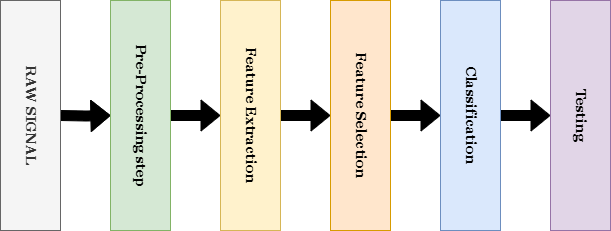
\includegraphics[width=0.75\linewidth]{Diagrams/icbmintro.drawio.png}
    \caption{System Architecture}
    \label{fig:sysarch}
\end{figure}
\begin{multicols}{2}

The above diagram ~\ref{fig:sysarch} shows the overall system architecture. The flow contains 6 steps (1) Data Acquisition using microphones $\rightarrow$ Raw Signal, (2) Pre-processing, (3) Feature Extraction, (4) Feature Selection, (5) Classification $\rightarrow$ SVM, (6) Testing and Validation.
The rest of this report is organized as follows. Section~\ref{sec:daq} describes the data acquisition setup and recording protocol. Section~\ref{sec:preprocess} summarizes the preprocessing steps used prior to decomposition. Section~\ref{sec:features} outlines the feature extraction and selection methods, and Section~\ref{sec:classification} describes the classification strategy. Experimental results and analysis are reported in Section~\ref{sec:results}, followed by conclusions and directions for future work in Section~\ref{sec:conclusion}. The DAQ setup and specific implementation details follow the experimental design in \cite{Verma2016}.

\section{Data Acquisition (DAQ) System}
\label{sec:daq}

This study used acoustic recordings to capture machine condition signatures. The DAQ choices focused on reproducibility and on maximizing signal quality while keeping the setup simple.

\subsection{Hardware and placement}
\begin{itemize}
  \item \textbf{Microphones:} Microphones were used to preferentially pick up sound directed toward each sensor and to reduce off-axis ambient noise.
  \item \textbf{DAQ hardware:} Recordings were acquired using a National Instruments NI-9234 dynamic signal acquisition module (four channels, 24-bit) connected via an NI-9172 chassis to a PC running LabVIEW for capture and storage. This setup allows up to four simultaneous microphone channels at high sample rates.
  \item \textbf{Sensor distance:} Empirical tests showed the cleanest and loudest captures when the microphone was placed approximately \textbf{1.5 cm} from the machine surface; this distance was used consistently for all recordings.
\end{itemize}
\subsection{Recording procedure}
\begin{itemize}
  \item \textbf{Duration \& sampling:} Each recording is 5 seconds long sampled at 50 kHz and stored as 24-bit PCM. Thus each raw file contains 250,000 samples.
  \item \textbf{Candidate positions:} To perform Sensitive Position Analysis (SPA) the machine was sampled at multiple candidate locations (the original study used 24 positions) so that a robust ranking of sensor positions could be obtained.
\end{itemize}
\subsubsection{Preliminary observations}
Practical tests revealed:
\begin{itemize}
    \item Microphones placed at roughly {1.5}{cm} from the machine provided stronger signals and reduced background contamination.
    \item Acoustic useful content predominantly lies below {12}{kHz} for the compressor under study \cite{Verma2016}; therefore, pre-processing included a high-pass filter (to remove fan noise) and a low-pass filter at {12}{kHz}.
    \item A clipping strategy (segment selection) with overlap helps to choose the most stable portion of each recording for robust analysis (detailed in Section~\ref{sec:preprocess}).
\end{itemize}
\section{Pre-Processing}
\label{sec:preprocess}
\begin{itemize}
  \item \textbf{Useful bandwidth:} For this compressor, the informative and useful acoustic content lies largely below 12 kHz; accordingly, later processing uses a low-pass cutoff around 12 kHz and a high-pass filter near 400 Hz to remove known background hum noises.
  \item \textbf{Clipping} Each 5 s recording is split into 9, 1 s segments with 50\% overlap; the segment with the minimum standard deviation is selected for analysis to avoid transient spikes and to choose the most stable portion of the recording.
  \item \textbf{Smoothing \& normalization:} A simple moving-average smoother removes impulsive outliers, and a robust min–max style normalization (ignore 0.025\% extreme samples at both tails when computing min/max) is used so that scaling is not driven by rare outliers.
  \item \textbf{Storage \& labeling:} Store raw .dat (24-bit PCM) files to ensure later classification stages. Our dataset comprises 8 classes and 225 recordings each, resulting in a total of 1800 recordings. 
\end{itemize}
\begin{figure}[H]
    \centering
    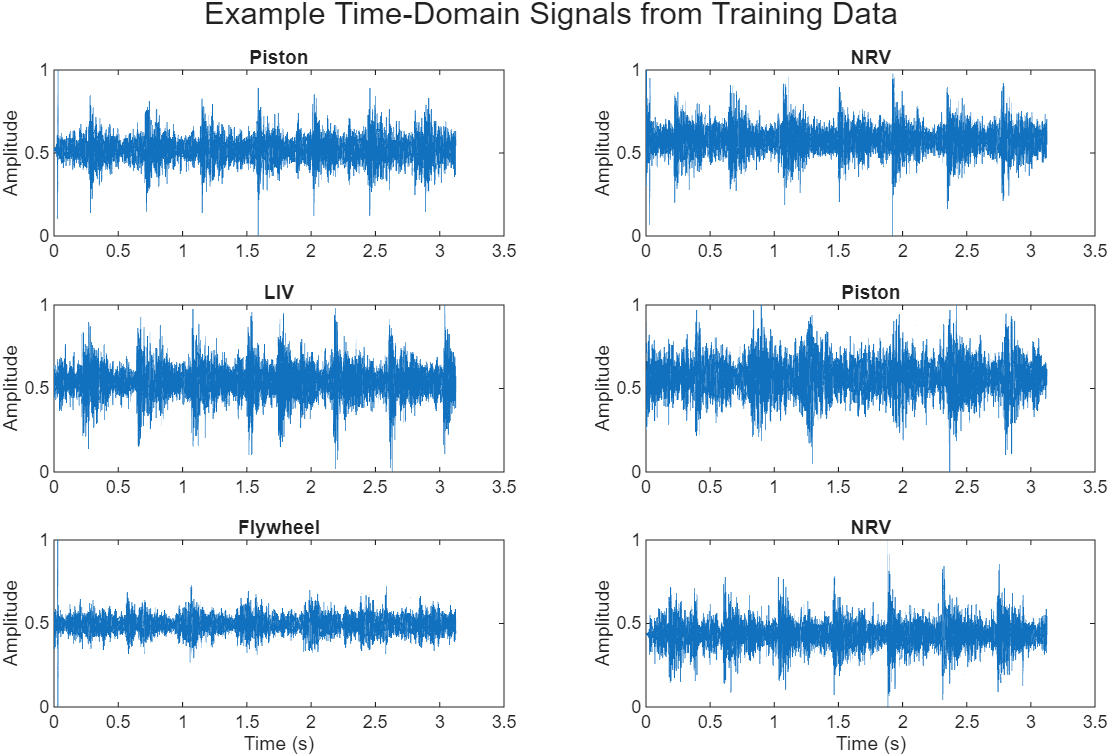
\includegraphics[width=1\linewidth]{Diagrams/preprocessing.png}
    \caption{Pre-processing steps}
    \label{fig:preprocessing steps}
\end{figure}
\section{Feature Extraction}
\subsection{Time Domain Features}
Time-domain features are found by looking directly at the original signal shape. These features include things like energy, changes in amplitude, and simple statistics such as the mean, root mean square (RMS), skewness, and kurtosis. Time-domain features are quick to calculate and help us understand the general vibration or sound patterns. In compressor monitoring, they are useful for spotting problems, since damage usually changes amplitude patterns or causes unusual spikes in the sound signal.
\subsection{Frequency Domain Features}
Frequency-domain features are calculated by using the Fourier Transform on the signal. This process helps us see how the signal's energy is spread out across different frequency ranges. In compressors, problems like leakage or worn valves can cause certain frequencies or harmonics to stand out. Features like spectral centroid, peak frequency, and band power can be more reliable than time-domain features, especially when faults show up as repeating or harmonic patterns in noisy data.
\subsection{Time Frequency Domain Features}
Time–frequency features show how the signal's frequency content changes over time. Unlike regular frequency analysis, this method helps us find short bursts or sudden changes in the signal. Since compressor signals often change over time, these features are important. By combining time and frequency details, time–frequency features can reveal patterns linked to certain faults, like brief impacts or sudden frequency shifts that standard Fourier analysis might miss.
\section{Feature Selection}
\label{sec:features}
Principal Component Analysis (PCA) is a dimensionality reduction technique that transforms a large set of correlated features into a smaller set of uncorrelated variables, known as principal components. A large collection of correlated features is reduced in dimensionality using Principal Component Analysis (PCA), which yields a smaller set of uncorrelated variables called principal components. Every component is ranked based on the variance it extracts from the dataset and is an orthogonal projection of the original features. This preserves the dominant structure of the data while enabling the compression of redundant and less informative features into a compact representation.
Using the entire feature set directly increases computational load and may result in lower classifier performance due to redundancy in the context of diagnosing acoustic faults, where hundreds of features are extracted across time, frequency, and wavelet domains.  We standardize the $286$-dimensional feature vectors, apply PCA to them, and project them into a lower-dimensional subspace in order to solve this.
 To assess the trade-off between dimensionality and classification accuracy, the number of retained components was changed from 10 to 200.  The Support Vector Machine (SVM) classifiers were then trained using these principal components as inputs in both One-Against-One (OAO) and One-Against-All (OAA) schemes.  This method guarantees quicker computation, lessens overfitting, and preserves the capacity to discriminate between compressor states that are healthy and those that are not.
% \begin{figure}[H]
%     \centering
%     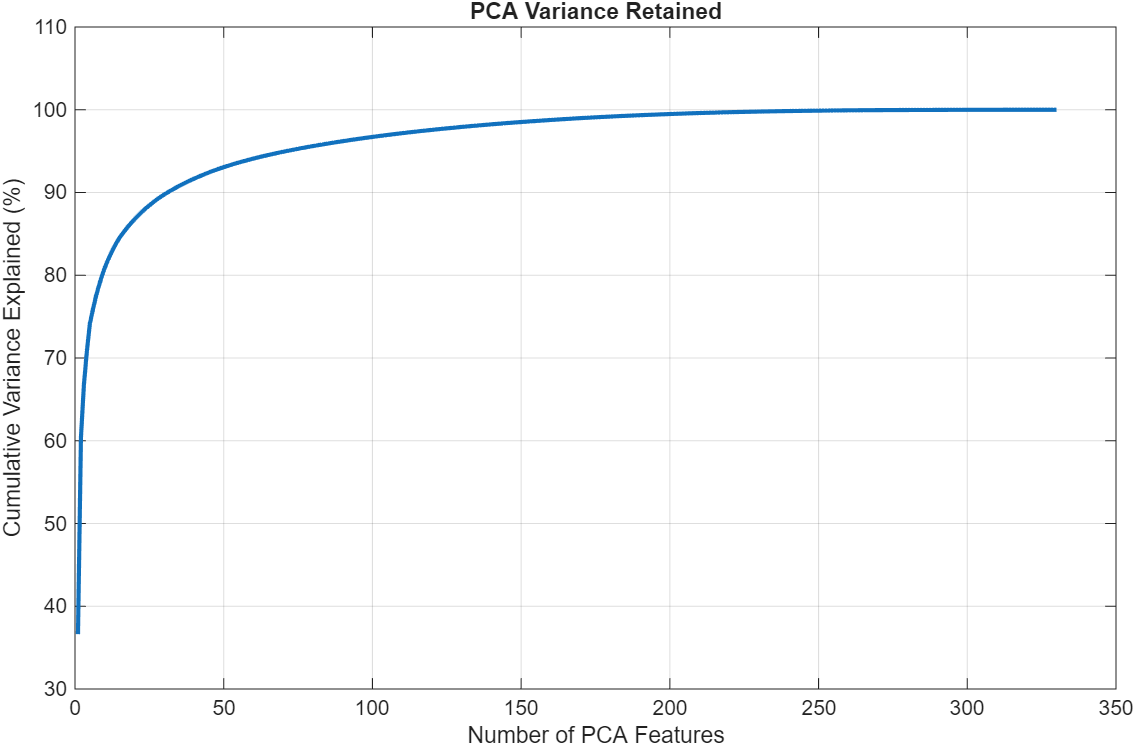
\includegraphics[width=1\linewidth]{Diagrams/pcavar.png}
%     \caption{PCA Variance}
%     \label{fig:PCA Variance}
% \end{figure}
\section{Use Case}

In this study, the proposed pipeline was tested on a single-stage reciprocating air compressor testbed with multiple seeded fault conditions.  The dataset consisted of acoustic recordings obtained from carefully selected sensor locations following Sensitive Position Analysis (SPA).  Each recording underwent pre-processing, decomposition, and transformation into a collection of statistical and signal-processing features.  A total of 286 features were extracted per segment, covering the time, frequency, and time-frequency domains.  The redundancy was then reduced using Principal Component Analysis (PCA), which compressed the feature space into a compact representation. 

\subsection{Classes, labels and Test-Train Split}

The dataset was labeled into eight distinct classes: one healthy state and seven different fault modes. These labeled feature vectors were split into training and testing sets, following the standard 70:30 test-train split, ensuring balanced representation across classes. 

The reduced feature set was then used to train Support Vector Machine (SVM) classifiers under both One-Against-All (OAA) and One-Against-One (OAO) schemes. This experimental setup provides a realistic use case where acoustic-based monitoring can distinguish multiple fault types with high reliability using only a single microphone location.


\begin{figure}[H]
    \centering
    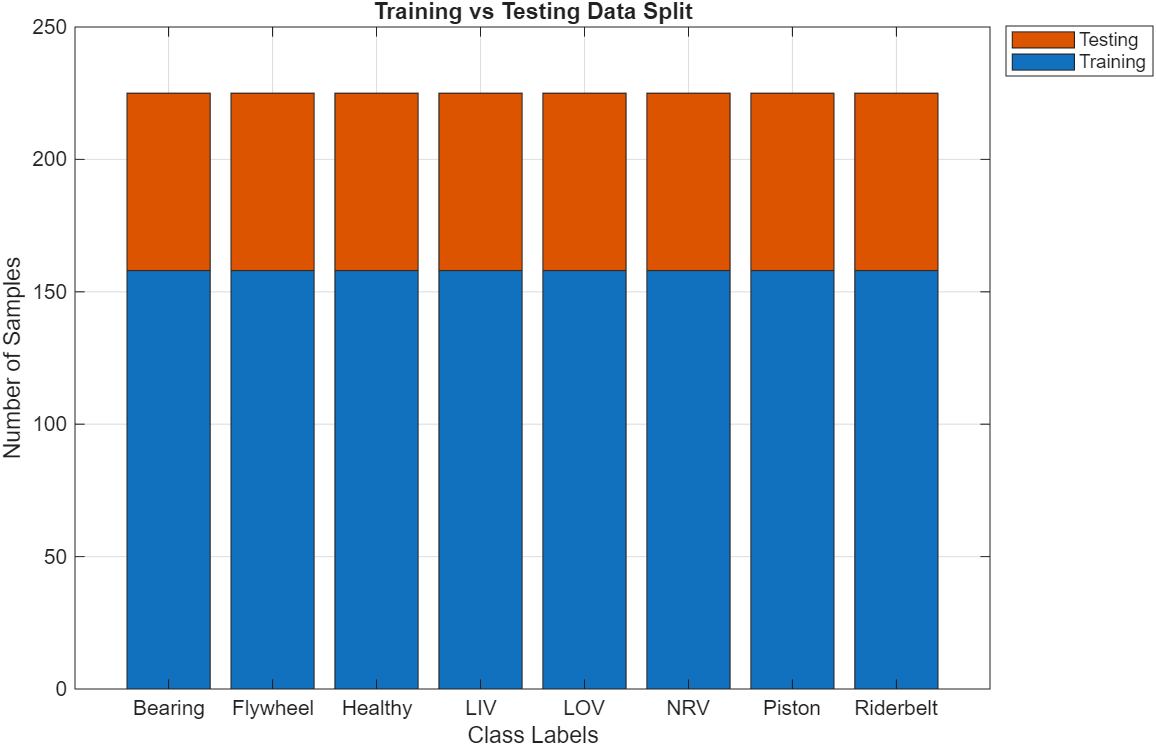
\includegraphics[width=1\linewidth]{Diagrams/split.png}
    \caption{Test Train Split}
    \label{fig:split}
\end{figure}
\begin{algorithm}[H]
\caption{Proposed Methodology for Acoustic Fault Diagnosis}
\label{alg:pipeline}
\KwIn{Acoustic dataset of compressor signals}
\KwOut{Predicted fault class}

\Begin{
    Load dataset into MATLAB using \texttt{audioDatastore}$\rightarrow$\;
    Assign labels for healthy and faulty conditions\;
    Preprocess signals$\rightarrow$\;
    Apply Wavelet Scattering Transform to extract coefficients$\rightarrow$\;
    Construct feature matrix$\rightarrow$\;
    Apply PCA for dimensionality reduction$\rightarrow$\;
    Split dataset into training and testing folds (5-fold CV)$\rightarrow$\;
    Train SVM classifiers$\rightarrow$One-Against-All (OAA) \&\ One-Against-One (OAO)$\rightarrow$ Evaluate classifiers using accuracy plots\;
}
\end{algorithm}

The proposed pipeline was implemented as discussed in the algorithm \ref{alg:pipeline} in MATLAB.  Acoustic recordings were pre-processed, segmented, and converted to features using the wavelet scattering transform.  This method uses cascaded wavelet filter banks to capture time-frequency information while removing irrelevant variability.  The extracted scattering coefficients were reduced with Principal Component Analysis (PCA) before being fed into Support Vector Machine (SVM) classifiers. 5 fold cross-validation was used to evaluate both the One-Against-All (OAA) and One-Against-One (OAO) classification schemes.

% \usepackage[ruled,vlined]{algorithm2e}



\section{Support Vector Machine (SVM)}
\label{sec:classification}


Support Vector Machines (SVM) were employed as the core classifiers for distinguishing compressor health and fault states. SVM is a powerful supervised learning technique that constructs hyperplanes in a high-dimensional feature space to maximize class distinctions. In this study, both \textbf{One-Against-All (OAA)} and \textbf{One-Against-One (OAO)} strategies were implemented for handling the multiclass nature of the problem.

\subsection*{Parameters}
The following parameters were selected for SVM training after empirical tuning:
\begin{itemize}
    \item \textbf{Kernel:} Radial Basis Function (RBF) kernel, chosen for its ability to model non-linear decision boundaries.
    \item \textbf{Box Constraint (C):} Optimized to balance margin width and classification error.
    \item \textbf{Kernel Scale:} Automatically optimized using MATLAB’s built-in heuristic.
    \item \textbf{Standardization:} Input features were standardized to zero mean and unit variance before training.
\end{itemize}

\subsection{Cross-Validation}
A \textbf{5-fold cross-validation} approach was used to evaluate model robustness and reduce overfitting. The dataset was randomly partitioned into 5 equal folds, with 4 folds used for training and 1 fold for testing in each iteration. The reported performance metrics are the average across all folds.

\subsection{Multiclass Classification}
Since the dataset consists of multiple classes (healthy + fault modes), two standard decomposition schemes were applied:
\subsubsection*{One-Against-All (OAA):} Constructs one classifier per class, distinguishing that class from all remaining classes.
\subsubsection*{One-Against-One (OAO):} Constructs pairwise classifiers between every possible pair of classes; final prediction is based on majority voting.

The comparative analysis of OAA and OAO allowed us to evaluate trade-offs between computational efficiency (OAA requires fewer models) and classification accuracy (OAO leverages pairwise discrimination).

\section{Results}
\label{sec:results}
The classification results for the proposed approach are summarized in 
Figures~\ref{fig:OAA_results} and~\ref{fig:OAO_results}. Both plots show the 
relationship between the number of retained PCA features and the achieved 
accuracy under 5-fold cross-validation for the two multiclass strategies.

\begin{figure}[H]
    \centering
    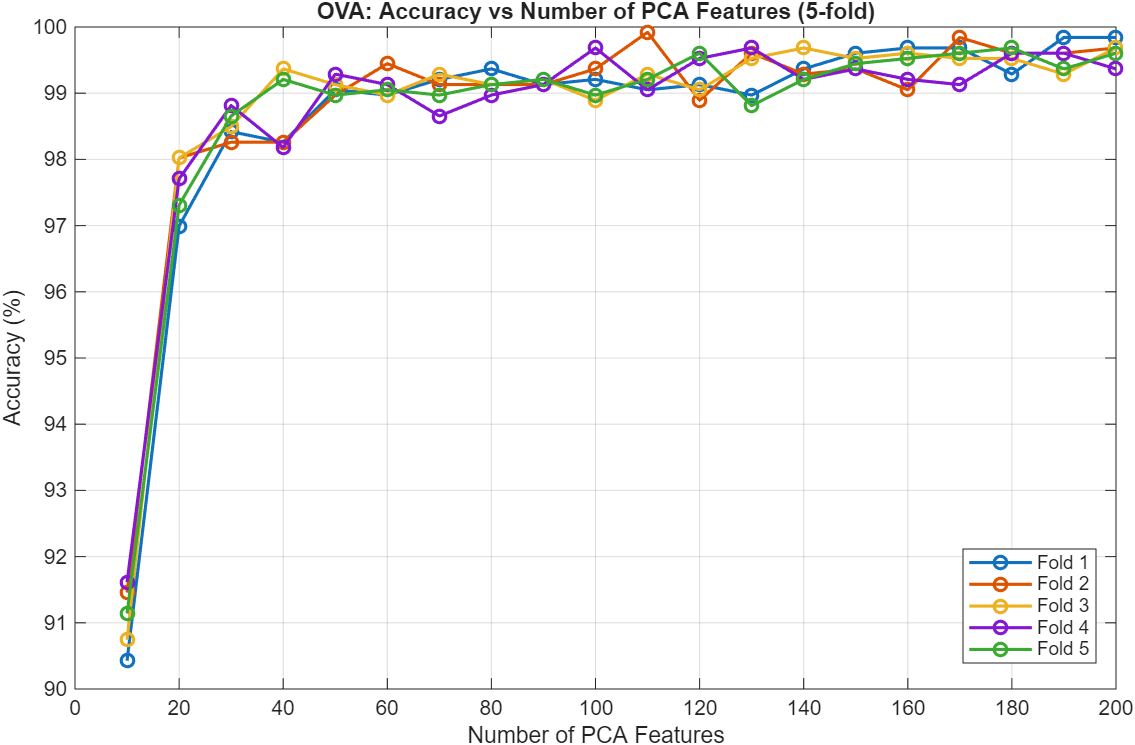
\includegraphics[width=1\linewidth]{Diagrams/res1.png}
    \caption{OAA: Accuracy vs Number of PCA Features (5-fold)}
    \label{fig:OAA_results}
\end{figure}

\begin{figure}[H]
    \centering
    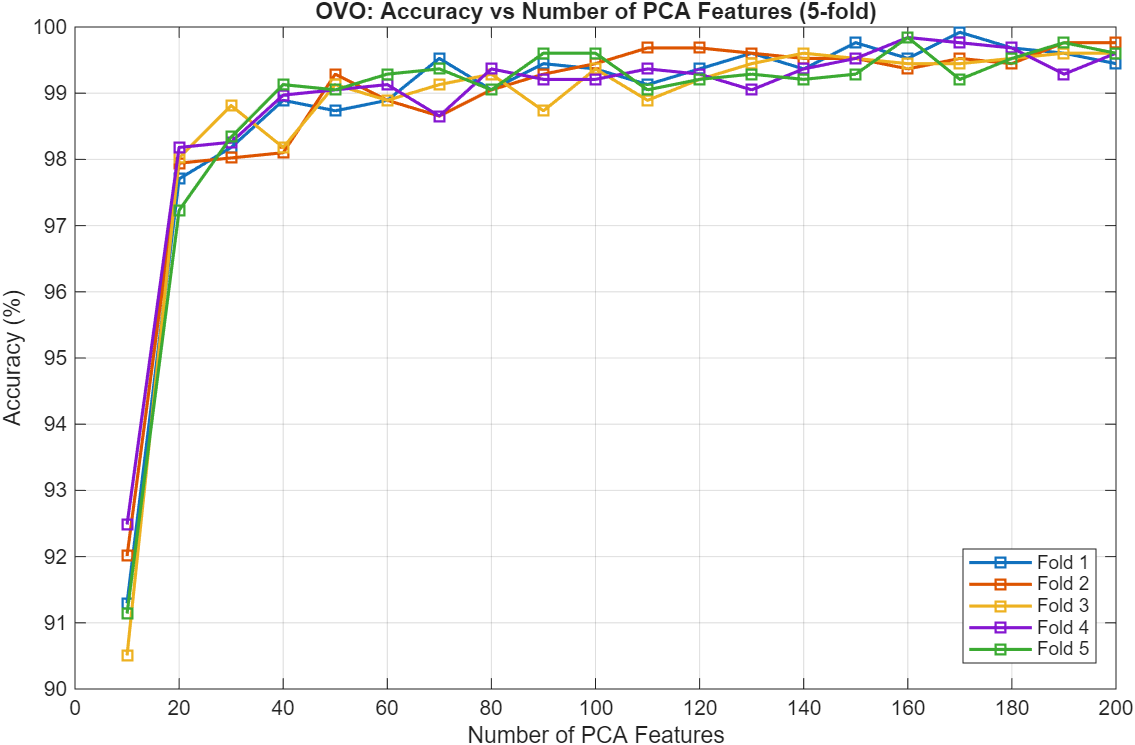
\includegraphics[width=1\linewidth]{Diagrams/res2.png}
    \caption{OAO: Accuracy vs Number of PCA Features (5-fold)}
    \label{fig:OAO_results}
\end{figure}

The results show that OAA and OAO schemes achieve high classification accuracy when the number of PCA components exceeds 40.  Accuracy increased from 91\% (with few components) to over 98\% when 40-60 features were used, gradually saturating.  For larger dimensions (more than 100 components), performance consistently exceeded 99.9\% across all folds.  
 The OAO approach outperformed OAA in terms of accuracy stability across folds, but both methods achieved near-perfect performance. 
 This confirms that PCA compresses the feature space while retaining discriminative information, and SVM classifiers can distinguish compressor states with a compact representation.

\section{Conclusion}
\label{sec:conclusion}
This study presented an end-to-end methodology for intelligent condition-based monitoring of air compressors via acoustic signals.  Using wavelet scattering features, PCA-based dimensionality reduction, and SVM classifiers, the system achieved near-perfect classification accuracy across multiple fault states.  Both OAA and OAO schemes performed well, with OAO producing slightly more consistent results across folds.  The results show that acoustic sensing, when combined with robust feature extraction and machine learning, provides a practical and accurate solution for fault diagnosis in industrial settings.

\begin{thebibliography}{1}
\bibitem{Verma2016}
N.~K. Verma, R.~K. Sevakula, S.~Dixit, and A.~Salour, ``Intelligent condition based monitoring using acoustic signals for air compressors,'' \emph{IEEE Transactions on Reliability}, vol.~65, no.~1, pp. 291--307, Mar. 2016. doi:10.1109/TR.2015.2459684.
\end{thebibliography}
\end{multicols}
\end{document}
